\section{等温间歇釜式反应器的计算(复合反应)}


\begin{frame}{平行反应}
    设在等温间歇釜式反应器中进行下列平行反应，P为目的产物
    \vspace{-2pt}
    $$\begin{array}{l}
        \mathrm{A} \longrightarrow \mathrm{P}, \quad r_{\mathrm{P}}=k_{1} c_{\mathrm{A}} \\
        \mathrm{A} \longrightarrow \mathrm{Q}, \quad r_{\mathrm{Q}}=k_{2} c_{\mathrm{A}}
    \end{array}$$
    各反应组分的物料衡算式如下: 
    $$\begin{cases}
        V_{\mathrm{r}}(k_{1}+k_{2}) c_{\mathrm{A}}+\frac{\mathrm{d} n_{\mathrm{A}}}{\mathrm{d} t}=0\\
        -V_{\mathrm{r}} k_{1} c_{\mathrm{A}}+\frac{\mathrm{d} n_{\mathrm{P}}}{\mathrm{d} t}=0\\
        -V_{\mathrm{r}} k_{2} c_{\mathrm{A}}+\frac{\mathrm{d} n_{\mathrm{Q}}}{\mathrm{d} t}=0
    \end{cases}
    \quad \text{对于恒容均相系统}
    \begin{cases}
        (k_{1}+k_{2}) c_{\mathrm{A}}+\frac{\mathrm{d} c_{\mathrm{A}}}{\mathrm{d} t}=0\\
        -k_{1} c_{\mathrm{A}}+\frac{\mathrm{d} c_{\mathrm{P}}}{\mathrm{d} t}=0\\
        -k_{2} c_{\mathrm{A}}+\frac{\mathrm{d} c_{\mathrm{Q}}}{\mathrm{d} t}=0
    \end{cases}
    \begin{matrix}
        (1)\\
        (2)\\
        (3)
    \end{matrix}$$
    设$t=0$时，$c_\mathrm{A}=c_\mathrm{A0}$，$c_\mathrm{P}=0$，$c_\mathrm{Q}=0$，积分式(1)有
    $$c_{\mathrm{A}}=c_{\mathrm{A} 0} \exp [-(k_{1}+k_{2}) t] \quad \text{或}\quad t=\frac{1}{k_{1}+k_{2}} \ln \frac{c_{\mathrm{A} 0}}{c_{\mathrm{A}}} =\frac{1}{k_{1}+k_{2}} \ln \frac{1}{1-X_{\mathrm{A}}}$$
\end{frame}


\begin{frame}{平行反应}
    积分式(2)可得反应时间$t$时目的产物P的浓度
    $$c_{\mathrm{P}}=\frac{k_{1} c_{\mathrm{A} 0}}{k_{1}+k_{2}}\left\{1-\exp \left[-(k_{1}+k_{2}) t\right]\right\}$$
    由$c_{\mathrm{Q}}=c_{\mathrm{A} 0}-c_{\mathrm{A}}-c_{\mathrm{P}}$得
    $$c_{\mathrm{Q}}=\frac{k_{2} c_{\mathrm{A} 0}}{k_{1}+k_{2}}\left\{1-\exp \left[-(k_{1}+k_{2}) t\right]\right\}$$
    $$\frac{c_{\mathrm{P}}}{c_{\mathrm{Q}}}=\frac{k_{1}}{k_{2}}$$
    两种反应产物的浓度之比，在任何反应时间下均等于两个反应的速率常数之比。但要注意这个关系只有当各反应的速率方程形式相同时才成立。
\end{frame}


\begin{frame}{平行反应}
    \begin{columns}[c]
        \column{9cm}
        根据$c_{\mathrm{A}},c_{\mathrm{P}},c_{\mathrm{Q}}$浓度式可绘出示意图如图所示。
        
        由图可见，反应物A的浓度总是随反应时间的增加而减少，而反应产物P和Q的浓度则随反应时间的增加而增高。
        \column{4.5cm}
            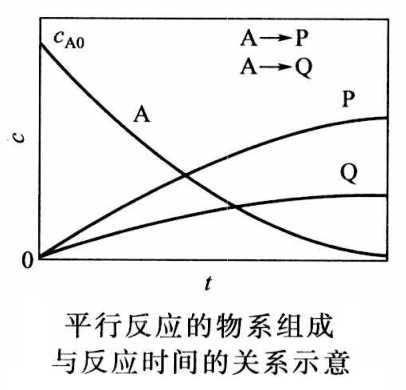
\includegraphics[width=4.5cm]{figs/fig3.2.png}
    \end{columns}
    以上是两个一级反应的情况，不难推广到M个一级反应同时进行情况
    $$c_{\mathrm{A}}=c_{\mathrm{A} 0} \exp (-t \sum_{1}^{M} k_{i}) \qquad c_{i}=\frac{k_{\mathrm{i}} c_{\mathrm{A} 0}}{\sum_{1}^{M} k_{i}}[1-\exp (-t \sum_{1}^{M} k_{i})]$$
    反应时间确定后，即可确定必需的反应体积。
\end{frame}


\begin{frame}[t]{}
    \begin{example}
        在等温间歇釜式反应器中进行下列液相反应
        $$\mathrm{A}+\mathrm{B} \longrightarrow \mathrm{P}, \quad r_{\mathrm{P}}=2 c_{\mathrm{A}}~~ \mathrm{kmol} /(\mathrm{m}^{3} \cdot \mathrm{h})$$
        $$ 2 \mathrm{~A} \longrightarrow \mathrm{Q}, \quad r_{\mathrm{Q}}=0.5 c_{\mathrm{A}}^{2} ~~\mathrm{kmol} /(\mathrm{m}^{3} \cdot \mathrm{h})$$
        反应开始时A和B的浓度均等于2kmol/m$^3$，目的产物为P，试计算反应时间为3h时A的转化率和P的收率。
    \end{example}
\end{frame}


\begin{frame}{连串反应}
    设在等温间歇反应器中进行下列一级不可逆连串反应
    $$\mathrm{A} \stackrel{k_{1}}{\longrightarrow} \mathrm{P} \stackrel{k_{2}}{\longrightarrow} \mathrm{Q}$$
    由于同时进行两个独立反应，故需建立两个物料衡算式以描述其反应过程。现选A和P作为关键组分，仿照处理平行反应时所用的方法，不难得到以下两式
    $$-\frac{\mathrm{d} c_{\mathrm{A}}}{\mathrm{d} t}=k_{1} c_{\mathrm{A}}$$
    $$\frac{\mathrm{d} c_{\mathrm{P}}}{\mathrm{d} t}=k_{1} c_{\mathrm{A}}-k_{2} c_{\mathrm{P}}$$
    设$t=0$时，$c_\mathrm{A}=c_\mathrm{A0}$，$c_\mathrm{P}=0$，$c_\mathrm{Q}=0$，积分式(1)有
    $$c_{\mathrm{A}}=c_{\mathrm{A} 0} e^{-k_{1} t} \quad\text{或}\quad t=\frac{1}{k_{1}} \ln \frac{c_{\mathrm{A} 0}}{c_{\mathrm{A}}}=\frac{1}{k_{1}} \ln \frac{1}{1-X_{\mathrm{A}}}$$
\end{frame}


\begin{frame}{连串反应}
    \begin{columns}[c]
        \column{9cm}
        $$\frac{\mathrm{d} c_{\mathrm{P}}}{\mathrm{d} t}+k_{2} c_{\mathrm{P}}=k_{1} c_{\mathrm{A} 0} e^{-k_{1} t}$$
        这是一阶线性微分方程，结合初始条件解得
        $$c_{\mathrm{P}}=\frac{k_{1} c_{\mathrm{A} 0}}{k_{1}-k_{2}}\left(e^{-k_{2} t}-e^{-k_{1} t}\right)$$
        $$c_{\mathrm{Q}}=c_{\mathrm{A} 0}-c_{\mathrm{A}}-c_{\mathrm{P}}=c_{\mathrm{A} 0}[1+\frac{k_{2} e^{-k_{1} t}-k_{1} e^{-k_{2} t}}{k_{1}-k_{2}}]$$
        \column{4.5cm}
            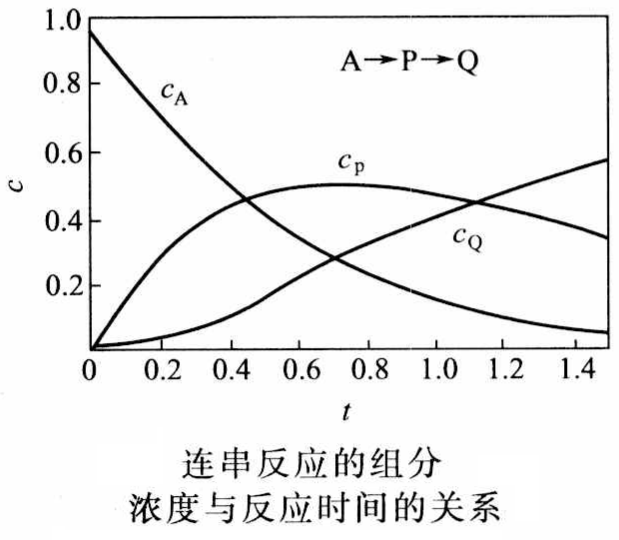
\includegraphics[width=4.5cm]{figs/fig3.3.png}
    \end{columns}
    由图可见，反应物A的浓度随反应时间的增加而减少，反应产物Q的浓度则随反应时间的增加而增高，而产物P的浓度先随时间增加而增加，后则随时间增加而降低，存在一最大值，这是连串反应的特点。
    
    反应时间短时，A的转化速率大于P转化成Q的速率，因而P的浓度随时间而增加。反应时间长时，P转化成Q的速率大于A转化成P的速率，P浓度下降。
\end{frame}


\begin{frame}{连串反应}
    当目的产物为P时，就需要控制反应时间，以使P的收率最大。
    
    将式$c_{\mathrm{P}}=\frac{k_{1} c_{\mathrm{A} 0}}{k_{1}-k_{2}}(e^{-k_{2} t}-e^{-k_{1} t})$对$t$求导，然后令$\mathrm{d}c_\mathrm{p}/\mathrm{d}t=0$可得最优反应时间
    $$t_{\mathrm{opt}}=\frac{\ln (k_{1} / k_{2})}{k_{1}-k_{2}}$$
    将$t_{\mathrm{opt}}$代回可求P的最大浓度。

    当目的产物为Q时，则反应时间越长，Q的收率越大。

    以上的讨论是针对包括两个一级反应的连串反应，其结论也可推广到更多反应时的场合，只要是中间产物，必存在极大浓度。对于非一级反应，可按上边的方法同样处理，只是大多数情况都很难获得解析解，需用数值解法。
    
    确定反应时间后，可根据式$V_\mathrm{r}=Q_0(t+t_0)$求反应体积。
\end{frame}


\begin{frame}[t]{}
    \begin{example}
        在间歇釜式反应器中等温下进行下列反应
        $$\mathrm{NH}_{3}+\mathrm{CH}_{3} \mathrm{OH} \stackrel{k_{1}}{\longrightarrow} \mathrm{CH}_{3} \mathrm{NH}_{2}+\mathrm{H}_{2} \mathrm{O}$$
        $$\mathrm{CH}_{3} \mathrm{NH}_{2}+\mathrm{CH}_{3} \mathrm{OH} \stackrel{k_{2}}{\longrightarrow}\left(\mathrm{CH}_{3}\right)_{2} \mathrm{NH}+\mathrm{H}_{2} \mathrm{O}$$
        这两个反应对各自的反应物均为一级，并已知反应温度下$k_2/k_1=0.68$，试计算一甲胺的最大收率和与其相应的氨转化率。
    \end{example}
\end{frame}
